\section{Bayesian Seroprevalence Analysis with Seroreversion Correction}
In a serial seroprevalence study conducted in Quebec, Canada by \cite{lewin2021sars} and \cite{lewin2022seroprevalence}, a procedure for seroreversion correction is applied in a non-Bayesian analysis. Here we begin by describing the dataset used in this analysis before illustrating the procedure used to adjust estimated cumulative incidences for seroreversion.
\subsection{Data}
The datasets used in \cite{lewin2021sars} and \cite{lewin2022seroprevalence} together can be viewed as one for a serial COVID-19 seroprevalence study in Quebec, Canada. For both phases of the study, numbers of antibody-positive samples as well as total number of samples are recorded for each of the three regions in Quebec: Montreal-Laval region, region surrounding Montreal-Laval, as well as other regions. Phase I of the study was conducted relatively early in the pandemic, and it collected samples obtained between May 25 and July 9, 2020. Phase II of the study contains samples collected from  January 25 to Mar 11, 2021.\\
\newline $ $
While we can use the data from phase I of the study to estimate regional cumulative incidences in Quebec between the beginning of the pandemic until around May 23, 2020 (accounting for the average 25 days between infection and when antibodies become detectable), simply repeating the same analysis using data from phase II of the study likely would not result in valid estimates of cumulative incidences between the beginning of the pandemic and the beginning of 2021. This is because there had already been almost a year since the beginning of the pandemic by the time when phase II samples were collected. Some of the individuals may have had a previous infection but had seroreverted by the time of sample collection. Consequently, the raw estimates may be lower than the true cumulative incidence of a given region. As a result, to account for seroreversion when analyzing data from phase II of the seroprevalence study, \cite{lewin2022seroprevalence} also conducted a seroreversion substudy. In particular, a number of the individuals who tested postive for SARS-Cov-2 antibodies during phase I of the study were tested again in 2021. The number of these individuals as well as the number of positive tests were recorded. The data from both phases of the study are summarized in \cref{tab:dat}.\\
\newline $ $
It is important to note that the phase II data presented here only concern the unvaccinated population. While data for both those who were and were not vaccinated are presented in \cite{lewin2022seroprevalence}, we have chosen to focus on the unvaccinated population since none of the vaccinated individuals had seroreverted at the time and so it is not necessary for adjust for seroreversion.

\begin{table}[]
\centering
\begin{tabular}{c|cc|cc|cc}
                           & \multicolumn{2}{c}{\textbf{Phase I}} & \multicolumn{2}{c}{\textbf{Phase II (unvaccinated)}} & \multicolumn{2}{c}{\textbf{Seroreversion substudy}}\\
                           & reactive      & tested      & reactive              & tested      & reactive              & tested        \\
                           \hline
Montreal-Laval             & 90            & 3061        & 48                    & 1925      & - & -          \\
Surrounding Montreal-Laval & 48            & 1925        & 128                   & 1422   & - & -             \\
Other                      & 35            & 2705        & 372                   & 4304          & - & -      \\
\hline
Total                      & 173           & 7691        & 715                   & 7304          &    77 & 109  
\end{tabular}
\caption{Seroprevalence data from \cite{lewin2021sars} and \cite{lewin2022seroprevalence}. Reactive indicates a positive test against SARS-Cov-2 IgG.}
\label{tab:dat}
\end{table}
\subsection{Adjusting for seroreversion}
omg

\subsection{Model formulation}
To maintian nice properties of Bayesian model while still accounting for seroreversion, can combine.

We can apply the approach in \cite{meyer2022adjusting} to the two datasets in \cite{lewin2021sars} and \cite{lewin2022seroprevalence} in one coherent Bayesian model that accounts for seroreversion. \\
\newline $ $
Let $s_{ij}$ denote the true seroprevalence in study $i$ and region $j$ ($i=1$ and $i=2$ correspond to first and second study, $j=1,j=2$ and $j=3$ correspond to Montreal-Laval, surrounding Montreal-Laval, and other regions). Let $P_{ij}$ denote the observed seroprevalances. Let $se, sp, sr$ denote sensitivity of test-kit, specificity of test-kit, as well as proportion of samples that has seroreverted (testing antibody-negative in 2021 but antibody-positive in 2020). Let $x_{ij}$ denote the total number of antibody-positive samples in region $j$ at study $i$, and $n_{ij}$ denote the total number of samples in region $j$ at study $i$. Finally, let $x_r$ and $n_r$ denote the total number of samples that seroreverted and the total number of samples in the seroreversion substudy. \\
\newline $ $
The model can then be written as
\[
s_{1j} &\sim \distBeta(1,1) \quad \forall j \in \{1,2,3\}\\
s_{2j} &\sim \distBeta(1, 1)_{\{ sr \times s_{1j} , 1 \}} \quad \forall j \in \{1,2,3\}\\
se &\sim \distBeta(205, 29)\\
sp &\sim \distBeta(288, 2)\\
sr &\sim \distBeta(32, 77)\\
p_{1j} &= s_{1j} \times se + (1 - s_{1j}) \times (1 - sp) \quad \forall j \in \{1,2,3\}\\
p_{2j} &= (s_{2j} - sr \times s_{1j}) \times se + (1 - (s_{2j} - sr \times s_{1j})) \times (1 - sp) \quad \forall j \in \{1,2,3\}\\
x_{ij} \given n_{ij}, p_{ij} &\distind \distBinom(n_{ij}, p_{ij}), \quad \forall i \in\{1,2\}, \quad j \in \{1,2,3\}.
\]
Following the notation from the previous section, the density of the target posterior distribution is given by
\[
p(S, se, sp, sr \given X, N) = \frac{1}{Z}p(se)p(sp)p(sr)\prod_{i=1}^3\prod_{j=1}^2 p(s_{ij})p(x_{ij}\given sp, se, sr, s_{ij}).
\]
Note that for observed seroprevalences in the first study, we adjust for test sensivitity and test specificity (Following the setup in \cite{meyer2022adjusting}. We'll likely use the same prior on $se$ and $sp$ here). For observed seroprevalences in the second study, we adjust for both test sensivitity and test specificity as well as seroreversion. Namely, we also include the proportion that have seroreverted since the first study using information from the seroreversion substudy. This combines the setup in \cite{lewin2022seroprevalence} and \cite{meyer2022adjusting}: we first substract the proportion that have seroreverted from the true seroprevalence and then adjust for test-kit performance. This is because the test-kit only has a chance at detecting antibodies if the subject has not seroreverted. To ensure we do not run into negative seroprevalence estimates, we truncate $s_{21}, s_{22}, s_{23}$ accordingly.\\
\newline $ $
Altogether, this can give us an estimate of the seroprevalance in Quebec, Canada in January to March 2021 adjusting for test-kit performance as well as seroreversion.\\
\newline $ $
We can compare the results from this above Bayesian model to those from \cite{lewin2022seroprevalence} (which is not Bayesian and does not account for test-kit performance) as well a frequentist equivalence of the above Bayesian model using the same data. We can use these results to check if the claims from \cite{lewin2022seroprevalence} still hold under this different dataset, as well as to explore potential reasons as to why they do or do not hold.\\
\newline $ $
It turns out that the intervals constructed from \cite{rosenberg2020cumulative} (the non-Bayesian analysis that \cite{meyer2022adjusting} compared to) is just by using the $95\%$ confidence interval endpoints for test sensitivity and specificity to correct for the true seroprevalence using $p = s \times se + (1-s) \times (1-sp)$.

\begin{table}[]
\centering
\label{tab:results}
\begin{tabular}{c|ccc}
                           & \multicolumn{3}{c}{\textbf{Raw result}}                                        \\
                           & mean                & lowerbound             & upperbound             \\
Montreal-Laval             & 0.136               & 0.120                  & 0.154                  \\
Surrounding Montreal-Laval & 0.090               & 0.076                  & 0.106                  \\
Other                      & 0.086               & 0.078                  & 0.095                  \\
\hline
                           & \multicolumn{3}{c}{\textbf{Adjusted for seroreversion}}                          \\
                           & mean                & lowerbound             & upperbound             \\
Montreal-Laval             & 0.145               & 0.125                  & 0.168                  \\
Surrounding Montreal-Laval & 0.097               & 0.080                  & 0.119                  \\
Other                      & 0.090               & 0.080                  & 0.102                  \\
\hline
                           & \multicolumn{3}{c}{\textbf{Adjusted for seroreversion and test-kit performance}} \\
                           & mean                & lowerbound             & upperbound             \\
Montreal-Laval             & 0.161               & 0.115                  & 0.177                  \\
Surrounding Montreal-Laval & 0.107               & 0.062                  & 0.120                  \\
Other                      & 0.100               & 0.056                  & 0.110                  \\
\hline
                           & \multicolumn{3}{c}{\textbf{Bayesian analysis adjusted for seroreversion and test-kit performance}}                                 \\
                           & median              & lowerbound             & upperbound             \\
Montreal-Laval             & 0.159               & 0.137                  & 0.183                  \\
Surrounding Montreal-Laval & 0.105               & 0.085                  & 0.125                  \\
Other                      & 0.096               & 0.082                  & 0.110                 
\end{tabular}
\caption{Summary of regional cumulative incidence point estimates and uncertainty intervals for all methods discussed. The first three non-Bayesian analyses contain the mean estimate as well as an uncertainty interval constructed from multiple $95$\% confidence intervals, and the last Bayesian analysis contain the median and equal-tailed $95$\% credible interval of the corresponding posterior distribution.}
\end{table}

\captionsetup[subfigure]{labelformat=empty}
\begin{figure}[ht!]
\centering
\begin{subfigure}[b]{\columnwidth} 
    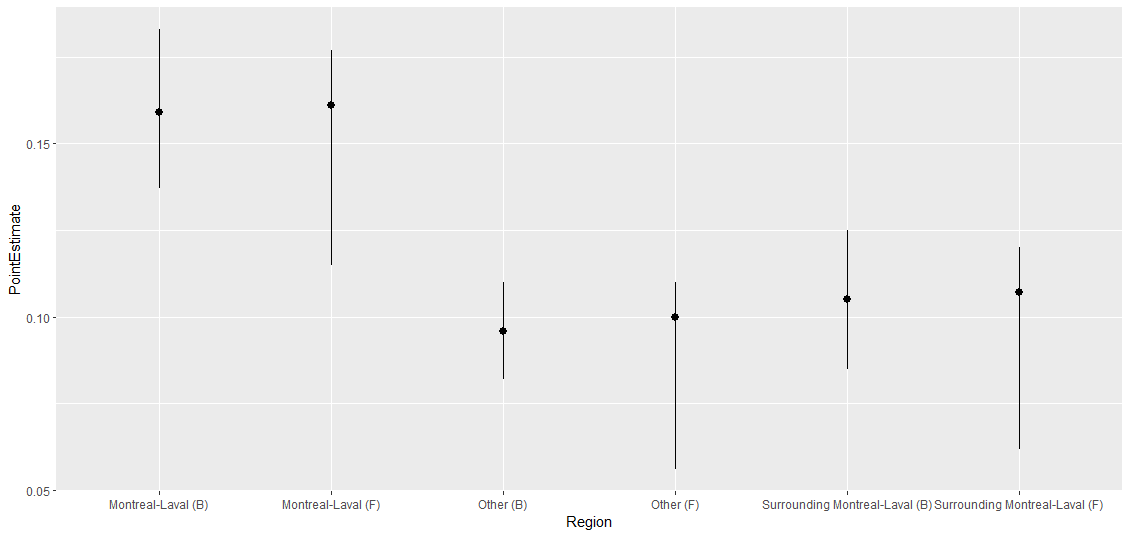
\includegraphics[width=\columnwidth]{../../plot/intervals.png}
    \caption{Comparison between uncertainty intervals for regional cumulative incidences between the Bayesian (B) and non-Bayesian (F) seroprevalence analyses, where both seroreversion and test-kit performance are accounted for.}
    \label{fig:intervals}
\end{subfigure}
\end{figure}

\subsection{Discussion of analysis results}